\begin{figure}
	\begin{subfigure}{\linewidth}
		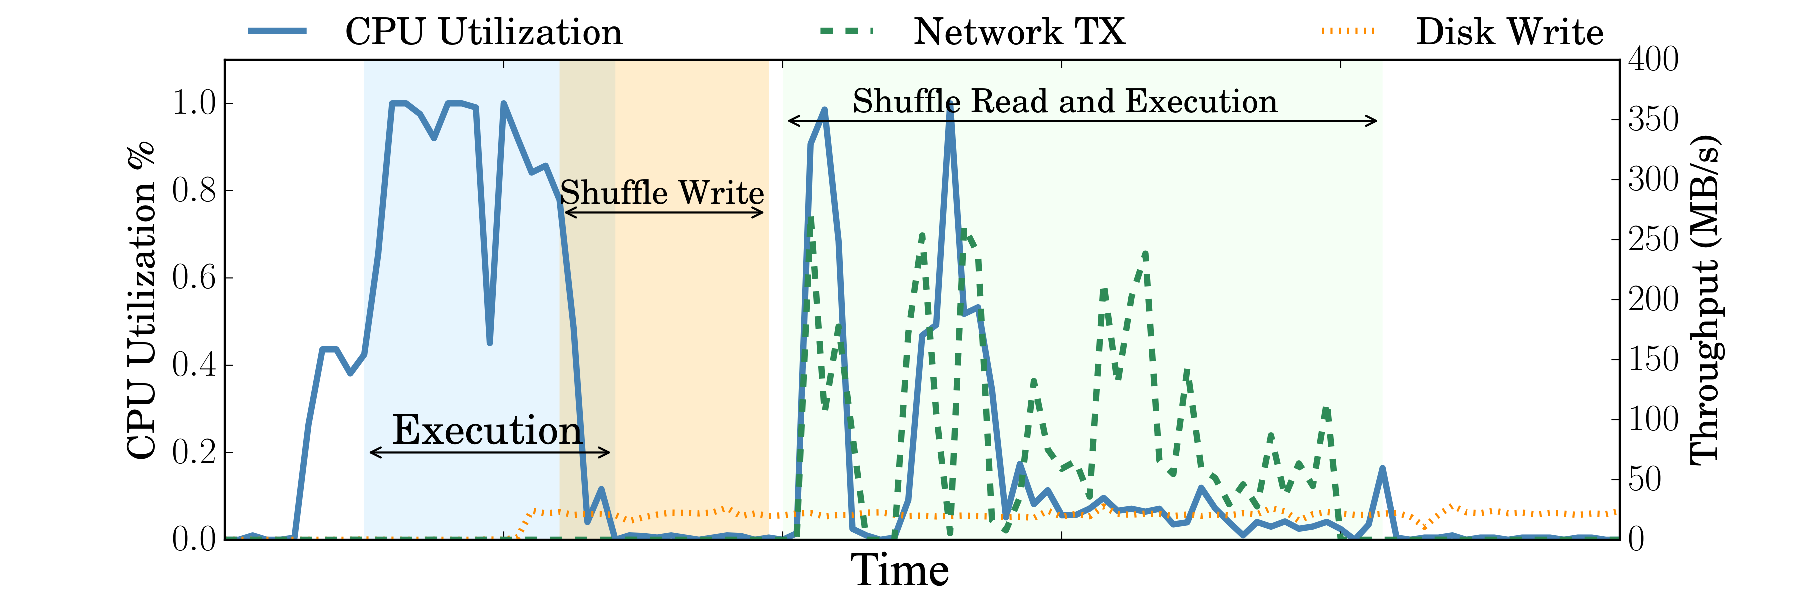
\includegraphics[width=\linewidth]{fig/util}
		\caption{Spark without SCache}
		\label{fig:util}
	\end{subfigure}
	% \vspace{-1em}
	\begin{subfigure}{\linewidth}
		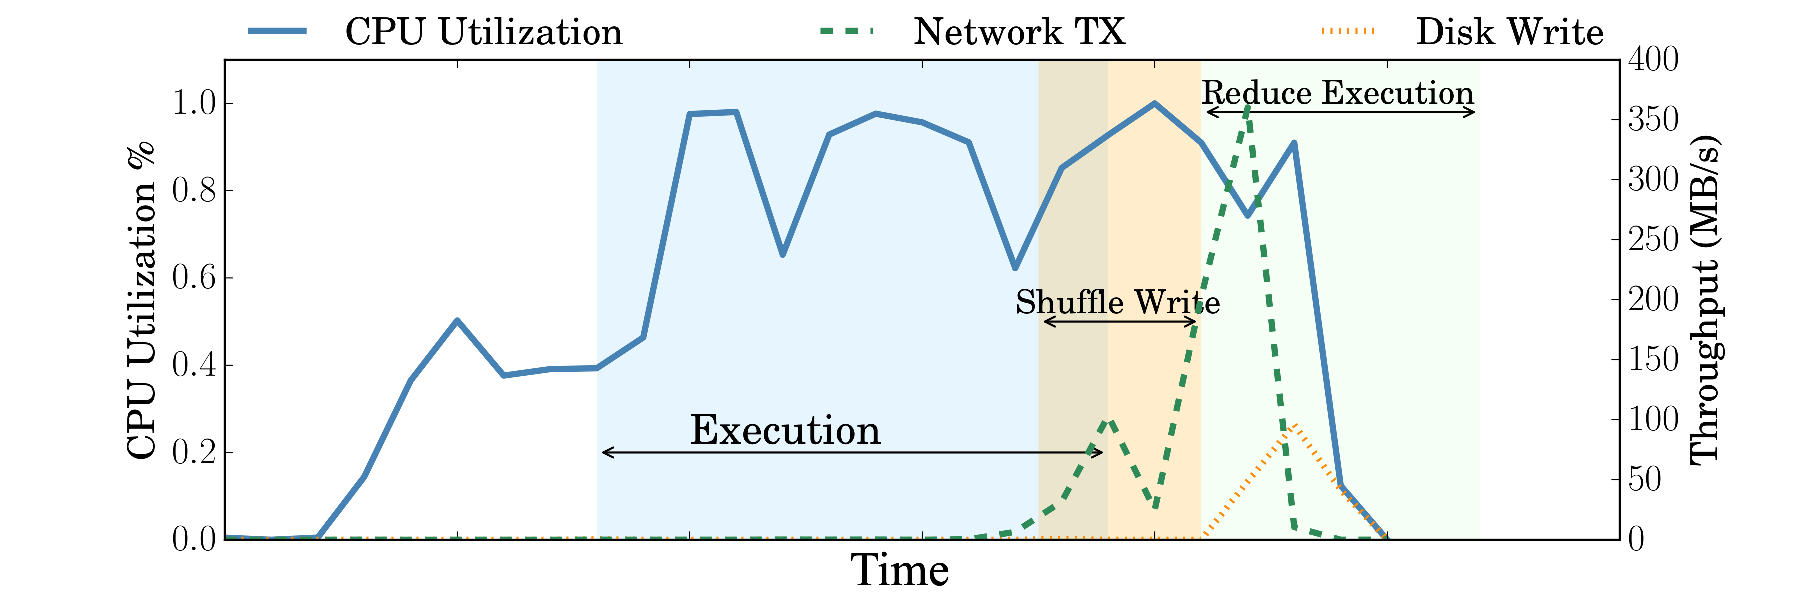
\includegraphics[width=\linewidth]{fig/scache_util}
		\caption{Spark with SCache}
		\label{fig:scache_util}
	\end{subfigure}
	\caption{CPU Utilization and I/O Throughput of a Node During a Spark Single Shuffle Application}
	\label{fig:simple_spark}
\end{figure}

\begin{figure*}
	\centering
	\begin{minipage}[t]{.5\textwidth}
	\begin{subfigure}{.5\linewidth}
		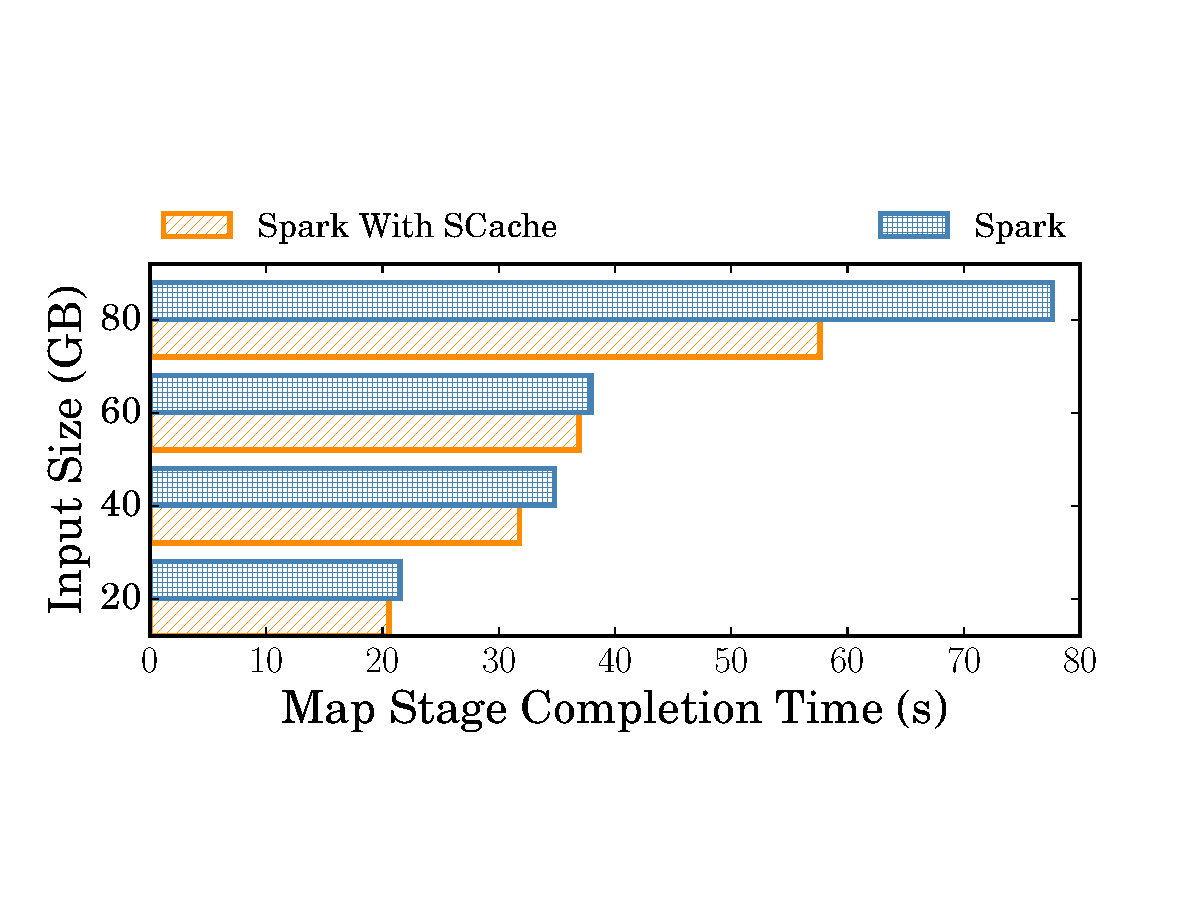
\includegraphics[width=\linewidth]{fig/groupbymapstage}
		\caption{Map Stage Completion Time}
		\label{fig:mapstage}
	\end{subfigure}
	\begin{subfigure}{.49\linewidth}
		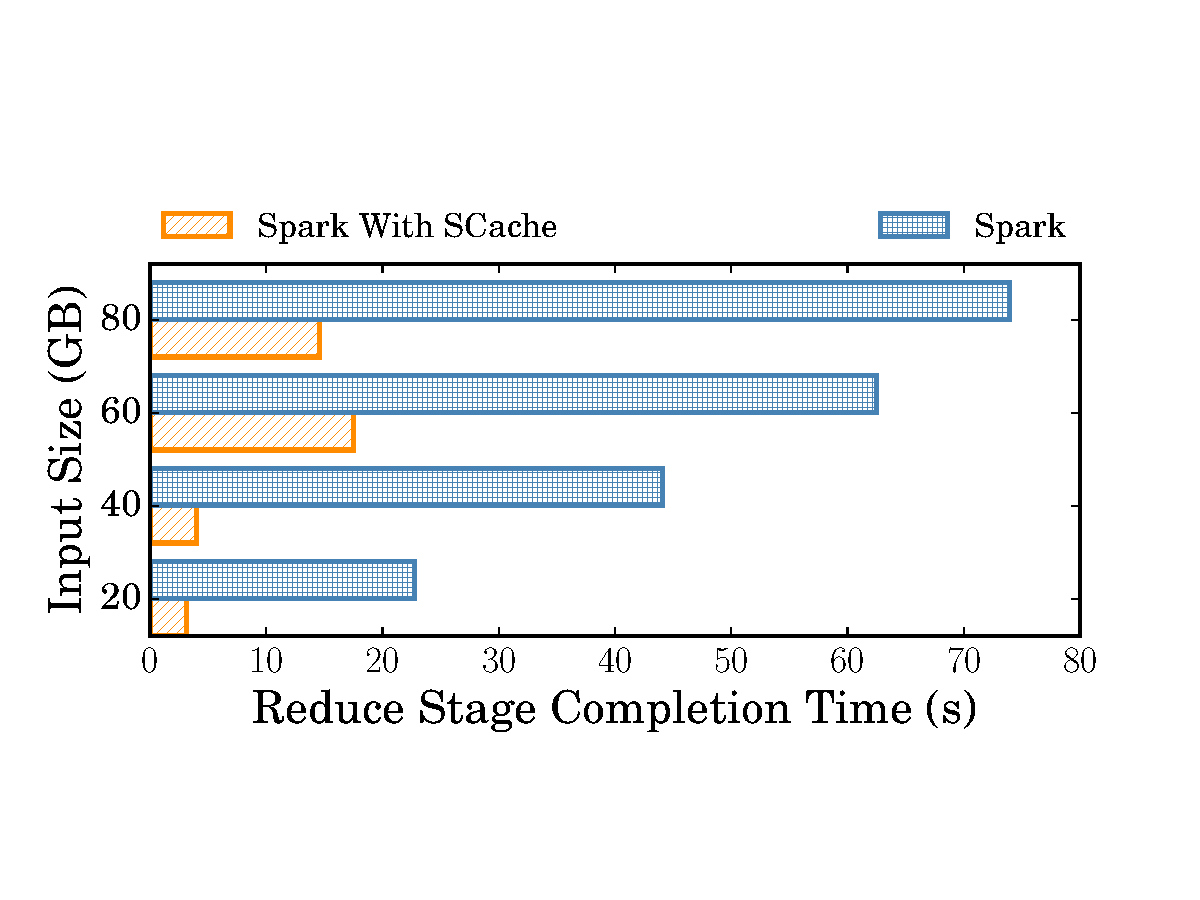
\includegraphics[width=\linewidth]{fig/groupbyreducestage}
		\caption{Reduce Stage Completion Time}
		\label{fig:reducestage}	
	\end{subfigure}
	\caption{Stage Completion Time of Single Shuffle Test}
	\label{fig:singleshuffle}
	\end{minipage}	
	\begin{minipage}[t]{.49\textwidth}
		\begin{subfigure}{.5\linewidth}
			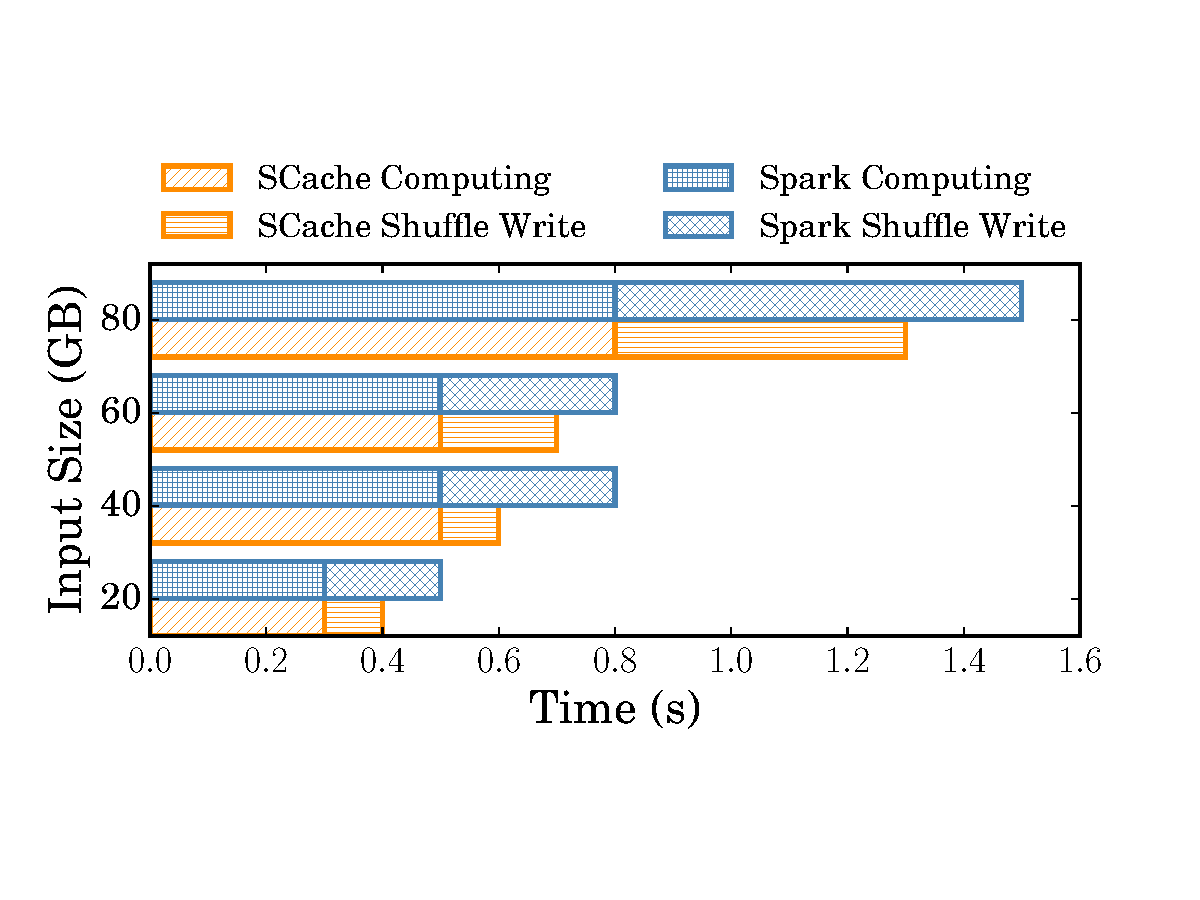
\includegraphics[width=\linewidth]{fig/groupbymaptask}
			\caption{Median Task in Map Stages}
			\label{fig:maptask}
		\end{subfigure}
		\begin{subfigure}{.49\linewidth}
			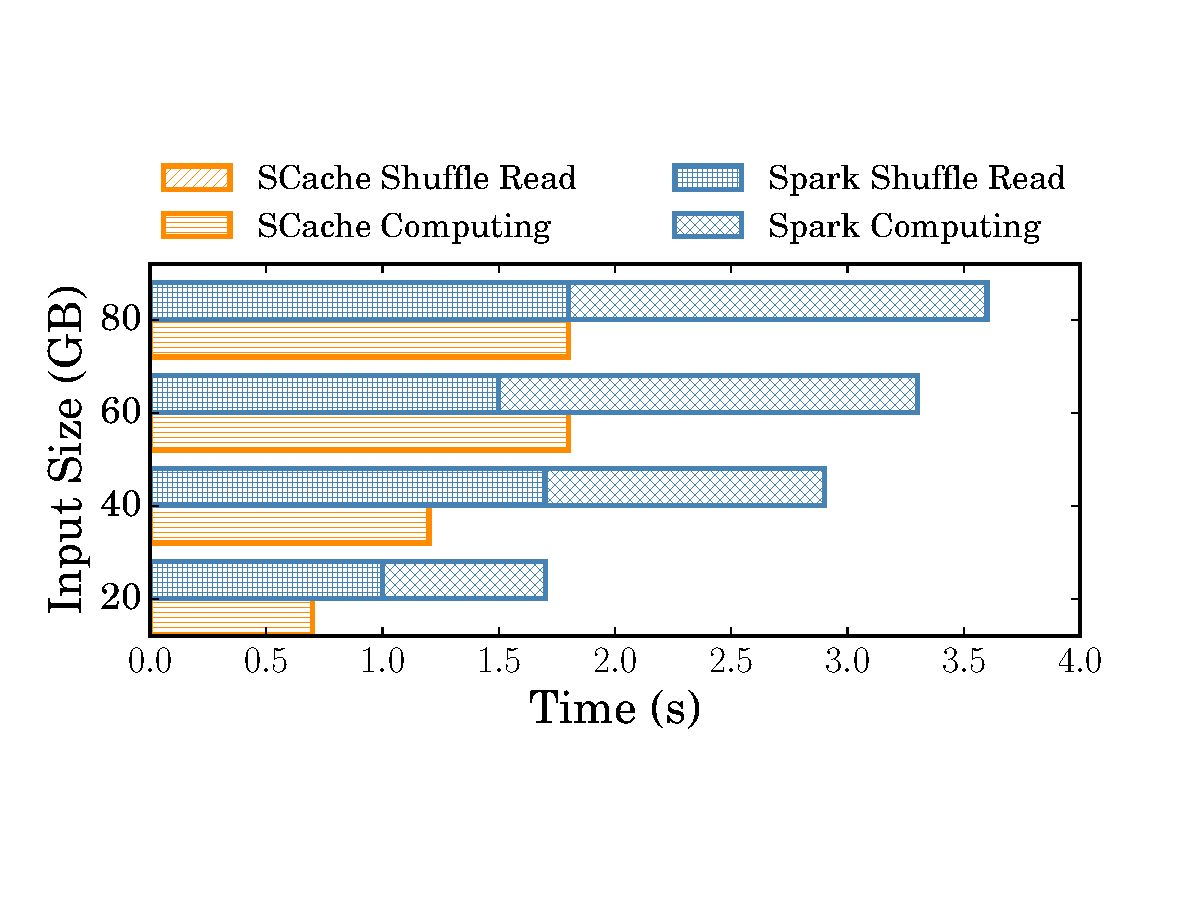
\includegraphics[width=\linewidth]{fig/groupbyreducetask}
			\caption{Median Task in Reduce Stages}
			\label{fig:reducetask}
		\end{subfigure}
		% \vspace{-1em}
		\caption{Median Task Completion Time of Single Shuffle Test}
		\label{fig:singleshuffletask}
	\end{minipage}	
\end{figure*}

\section{Evaluation}\label{evaluation}

% This section reveals the evaluation of SCache with comprehensive workloads and benchmarks which include common operations in the industrial big data analysis. 
{\color{black}
This section reveals a representative evaluation of SCache performance on both Spark and Hadoop MapReduce.
% To show the compatibility of SCache as a cross-framework plug-in, we implement and evaluate SCache on both Spark and Hadoop MapReduce. 
% We implement and evaluate SCache on Spark and Hadoop MapReduce, since they are the two most distributed computing frameworks using in industrial big data analysis.
In industrial big data, SQL-based big data technologies are widely used in these systems, such as data mining, predictive analytics, text analytics, and statistical analysis \cite{poess2017analysis}.
% SQL-Based Big Data Systems are widely used on industrial application.
% Because of the limited time and resource, 
To prove the performance gain of SCache in industry, 
we evaluate SCache with TPC-DS\footnote{http://www.tpc.org/tpcds/}.
TPC-DS is a standard benchmark which focuses on modeling industrial workload.
% TPC-DS, TPCx-BB, HiBench, BigDataBenchmark, and so on are popular standard big data benchmarks which evaluate big data systems.
% TPC-DS models queries and data maintenance of a retail product supplier and provides a representative evaluation of performance.
% We believe using TPC-DS is able to evaluate the performance of SCache in industry. 
% First, we evaluate the Spark with SCache in two different benchmarks.
% We run a Spark job with single shuffle to analyze hardware utilization and see the impacts of different components from the scope of a task to a job. 
% Then we use a recognized shuffle intensive benchmark --- Terasort to evaluate SCache with different data partition schemes.
% To prove the performance gain of SCache with a industrial production workload, we also evaluate Spark TPC-DS\footnote{https://github.com/databricks/spark-sql-perf} and present the overall performance improvement.
% In order to prove the performance gain of SCache with a real production workload, we also evaluate Spark TPC-DS\footnote{https://github.com/databricks/spark-sql-perf} and present the overall performance improvement.
% To prove the compatibility of SCache as a cross-framework plug-in, we implemented SCache on both Hadoop MapReduce and Spark. 
% Second, due to the simple DAG computing in Hadoop MapReduce, we only use Terasort as a shuffle-heavy benchmark to evaluate the performance of Hadoop MapReduce with SCache.
% Finally, we measure the overhead of weighted reservoir sampling. 
% In summary, SCache decreases ~$89\%$ time of Spark shuffle without introducing extra network transfer.
% More impressively, the overall completion time of TPC-DS can be improved ~$40\%$ on average by SCache.
%  applying the optimization from SCache.
In summary, SCache decreases ~$89\%$ time of Spark shuffle and improves ~$40\%$ of the overall completion time of TPC-DS on average.
Meanwhile, Hadoop MapReduce with SCache optimizes job completion time by up to $15\%$ and an average of $13\%$.
}


% Because a complex Spark application consists of multiple stages. The completion time of each stage varies under different input data, configurations and different number of stages. This uncertainty leads to the dilemma that dramatic fluctuation occurs in overall performance comparison. To present a straightforward illustration, we limit the scope of most evaluations in a single stage.


\subsection{Setup}\label{stepup}
% We modified Spark to enable shuffle optimization of SCache as a representative.
We use Spark version 1.6.2 and Hadoop MapReduce version 2.8.5.
The shuffle configuration of Spark is set to the default\footnote{http://spark.apache.org/docs/1.6.2/configuration.html}. 
We run the experiments on a 50-node m4.xlarge cluster on Amazon EC2.
% \footnote{http://aws.amazon.com/ec2/}. 
Each node has 16GB memory and 4 CPUs.
The network bandwidth of each node is about 300 Mbps.
% The network bandwidth provided by Amazon is insufficient. 
% Our evaluations reveal the bandwidth is only about 300 Mbps.
%  (see Figure \ref{fig:util}).

\subsection{Spark with SCache}\label{sparkscache}

\subsubsection{Simple DAG Analysis}\label{simpledag}
% As shown in Figure \ref{fig:scache_util}, we first run the same single shuffle test shown in Figure \ref{fig:util}. 
We first run Spark's \textit{GroupByTest} on Amazon EC2.
This job has 2 rounds of tasks for each node.
% We first run the same single shuffle test shown in Figure \ref{fig:util}. 
% For each stage, we run 5 rounds of tasks with different input size. 
As shown in Figure \ref{fig:simple_spark}, the hardware utilization is captured from one node during the job. 
Note that since the completion time of the job with SCache is about $50\%$ less than Spark without SCache, the duration of Figure \ref{fig:scache_util} is only half of Figure \ref{fig:util}.
As shown in \ref{fig:util}, the network transfer of shuffle data introduces an explicit I/O delay during \textit{shuffle read}.
And the several bursts of network traffic in \textit{shuffle read} result in network congestion.
As shown in Figure \ref{fig:scache_util}, an overlap among CPU, disk, and network can be easily observed. 
It is because the decoupling of shuffle prevents the computing resource from being blocked by I/O operations. 
On the one hand, the decoupling of shuffle write helps free the slot earlier, so that it can be re-scheduled to a new map task.
On the other hand, with the help of shuffle pre-fetching, the decoupling of shuffle read significantly decreases the CPU idle time at the beginning of a reduce task.
At the same time, SCache manages the hardware resources to store and transfer shuffle data without interrupting the computing process.
As a result, the utilization and multiplexing of hardware resource are increased, thus improving the performance of Spark. 

% The performance evaluation in Figure \ref{fig:singleshuffletask} shows the consistent results with our observation of hardware utilization. 
% For each stage, we pick the task that has median completion time. 
In the map stage, the disk operations are replaced by the memory copies to decouple the shuffle write. 
It helps eliminate $40\%$ of shuffle write time (Figure \ref{fig:maptask}), which leads to a $10\%$ improvement of map stage completion time in Figure \ref{fig:mapstage}. 
% Note that the shuffle write time can be observed even with the optimization of SCache. 
% The reason is that before moving data out of Spark's JVM, the serialization is inevitable and CPU intensive \cite{makingsense}. 
In the reduce stage, most of the shuffle overhead is introduced by network transfer delay. 
By doing shuffle data pre-fetching, the explicit network transfer is perfectly overlapped in the map stage. 
% By doing shuffle data pre-fetching based on the pre-scheduling results, the explicit network transfer is perfectly overlapped in the map stage. 
% With the help of the co-scheduling scheme, SCache guarantees that each reduce task has the benefit of shuffle pre-fetching. 
% The in-memory cache of shuffle data further reduces the shuffle read time. 
As a result, the combination of these optimizations decreases ~$100\%$ overhead of the shuffle read in a reduce task (Figure \ref{fig:reducetask}). 
In addition, the heuristic algorithm can achieve a balanced pre-scheduling result, thus providing ~$80\%$ improvement in reduce stage completion time (Figure \ref{fig:reducestage}).

Overall, SCache can help Spark decrease by ~$89\%$ overhead of the whole shuffle process. 

% \subsubsection{Terasort}
% We also evaluate Terasort\footnote{http://sortbenchmark.org/YahooHadoop.pdf} --- a recognized shuffle intensive benchmark for distributed system analysis. 
% Terasort consists of two consecutive shuffles. 
% The first shuffle reads the input data and uses a hash partition function for re-partitioning. 
% As shown in Figure \ref{fig:terasort}, Spark with SCache runs 2 $\times$ faster during the reduce stage of the first shuffle, which is consistent with the results in Section \ref{simpledag}. 
% It further proves the effectiveness of SCache's optimization.

% The second shuffle of Terasort partitions the data through a Spark RangePartitioner. 
% % As the range bounds set by range partitioner almost match the same pattern of the first shuffle, almost $93\%$ of input data is from one particular map task for each reduce task. So we take the second shuffle as an extreme case to evaluate the scheduling locality for SCache.
% In the second shuffle, almost $93\%$ of input data of a reduce task is produced by one particular map task. 
% So we take the second shuffle as an extreme case to evaluate the heuristic locality swap of SCache.
% In this shuffle, Spark schedules a reduce task to the node that produces most input data. 
% By doing this, Spark minimizes the shuffle data through network. 
% At the same time, Figure \ref{fig:terashuffle} reveals that SCache produces exactly same network traffic as Spark. 
% It implies that the heuristic locality swap of SCache can obtain the best locality while balancing the load. 
\begin{figure*}
	\centering
	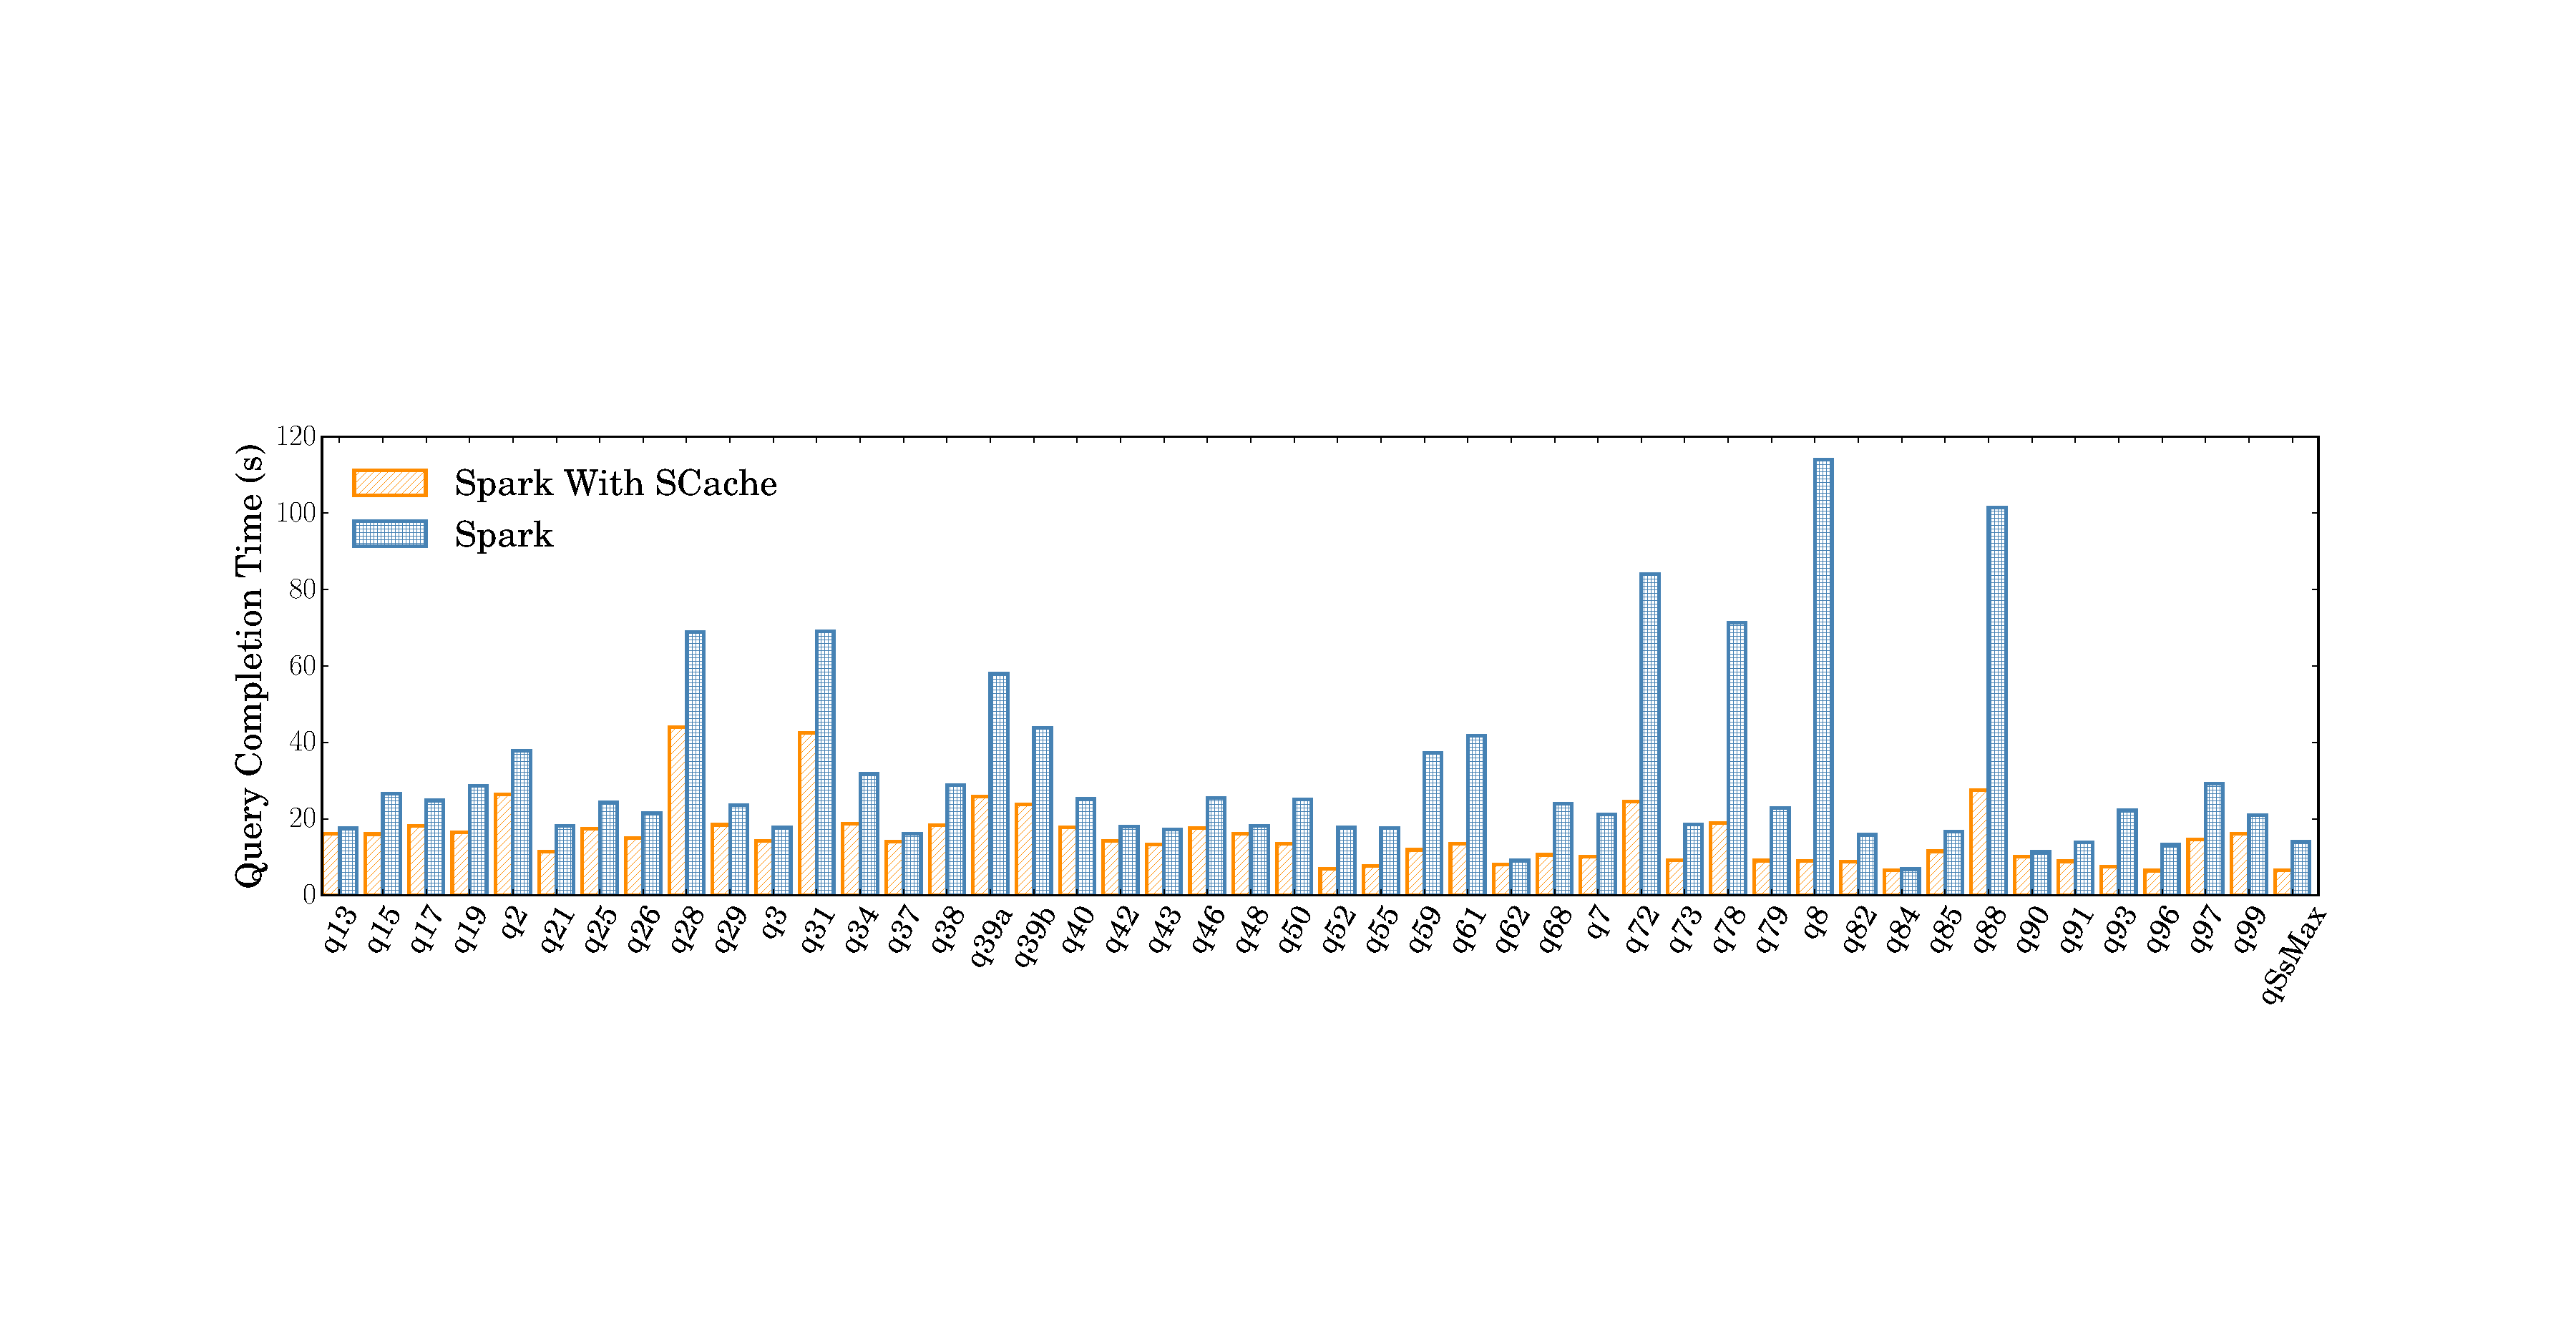
\includegraphics[width=.8\textwidth]{fig/tpcds}
	\caption{TPC-DS Benchmark Evaluation}
	\label{fig:tpcds}
	\vspace{-1em}
\end{figure*}

\subsubsection{Industrial Production Workload}
% We also evaluate some queries from TPC-DS\footnote{http://www.tpc.org/tpcds/}. 
% TPC-DS benchmark is designed for modeling multiple users submitting varied queries (e.g. ad-hoc, interactive OLAP, data mining, etc.). 
% TPC-DS contains 99 queries and is considered as the standardized industry benchmark for testing big data systems. 
TPC-DS\footnote{http://www.tpc.org/tpcds/} contains 99 queries and is considered as a standardized industry benchmark for testing big data systems. 
% We evaluate the performance of Spark with SCache by picking some of the TPC-DS queries with shuffle intensive attribute. 
As shown in Figure \ref{fig:tpcds}, the horizontal axis is query name and the vertical axis is query completion time. 
Note that we skip some queries due to the compatible issues. 
Spark with SCache outperforms the original Spark in almost all tested queries. 
Furthermore, in some shuffle-heavy queries, Spark with SCache outperforms original Spark by an order of magnitude. 
% It is because that those queries contain shuffle-heavy operations such as \textit{groupby}, \textit{union}, etc.
The overall reduction portion of query time that SCache achieved is $40\%$ on average. 
Since this evaluation presents the overall job completion time of queries, we believe that our shuffle optimization is promising.

\begin{figure}
	\centering
	\begin{subfigure}{.8\linewidth}
		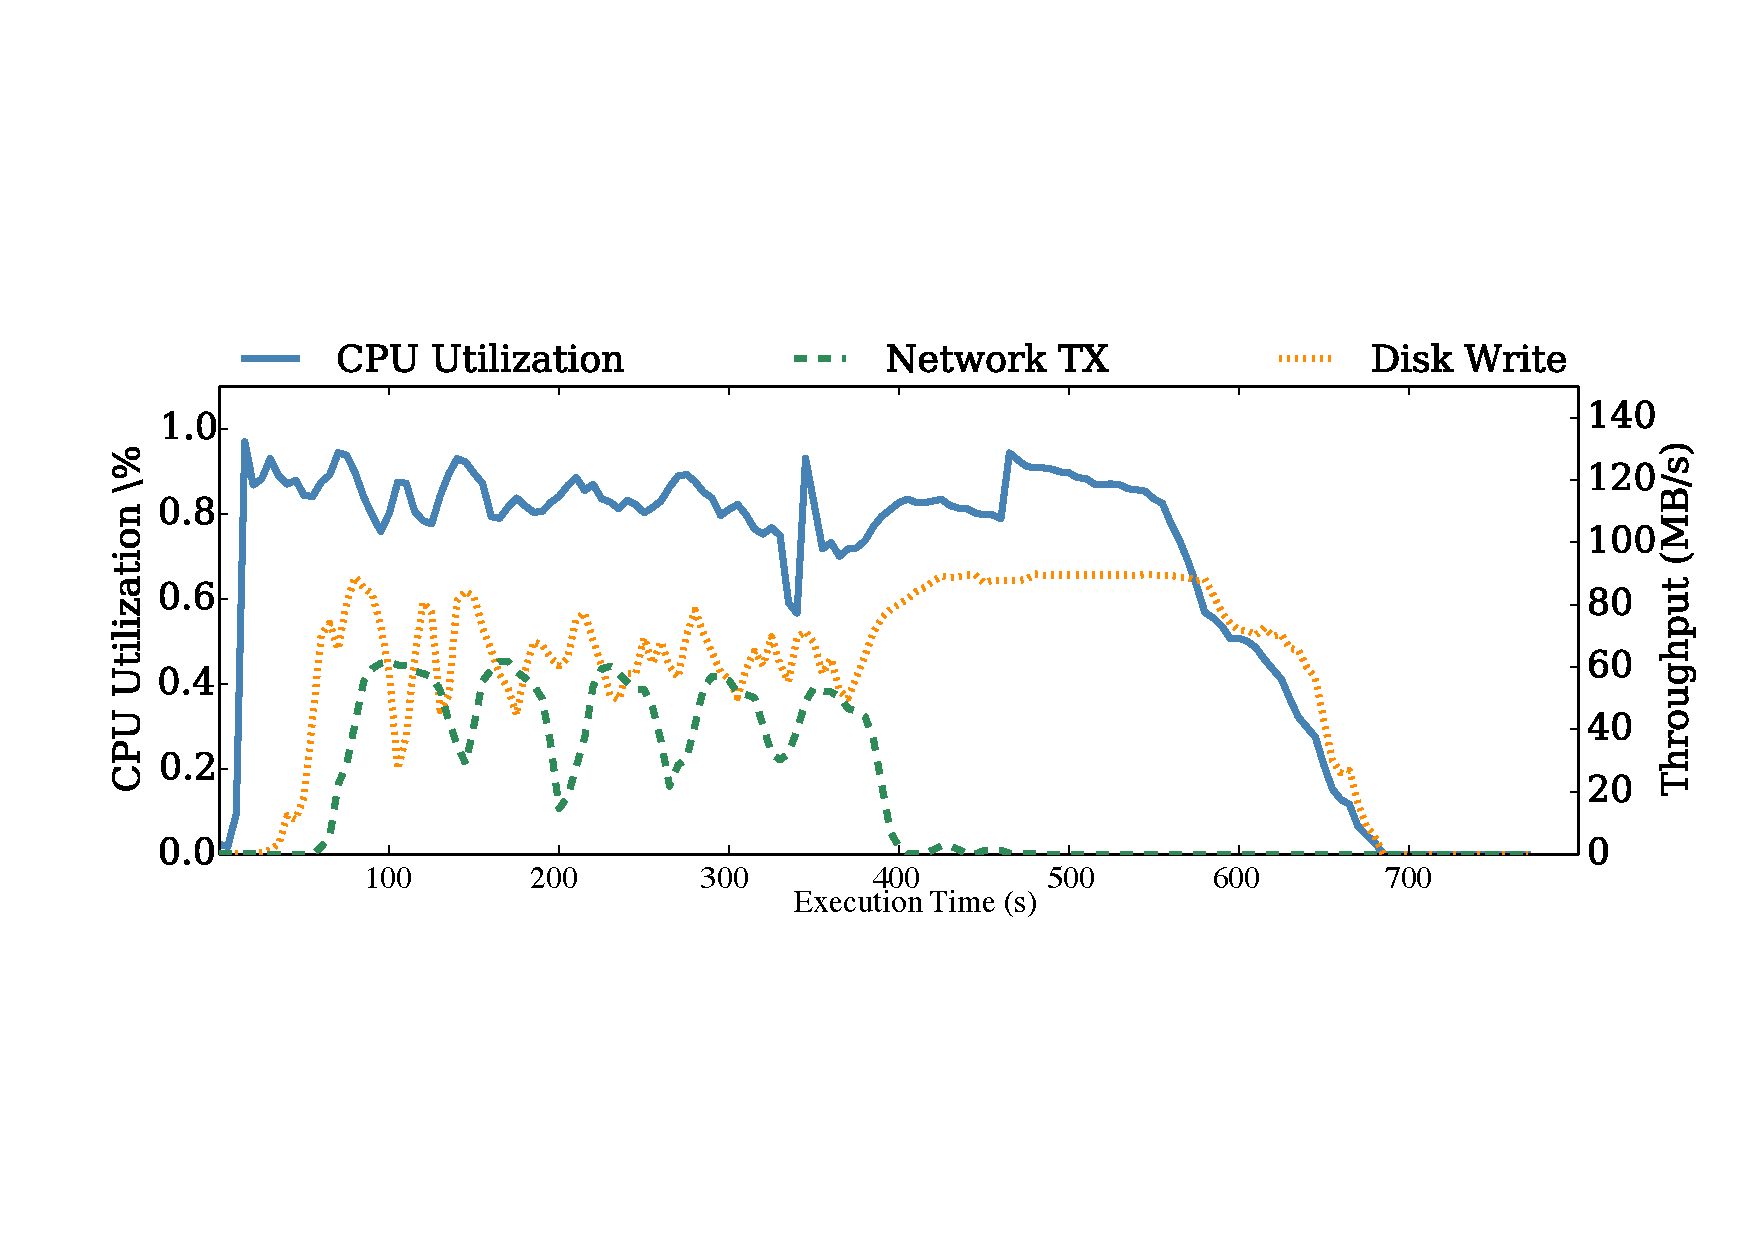
\includegraphics[width=\linewidth]{fig/hadoop_terasort_scache}
		\caption{\color{black}Hadoop MapReduce with SCache}
		\label{fig:hadoop_terasort_scache}
	\end{subfigure}
	\begin{subfigure}{.8\linewidth}
		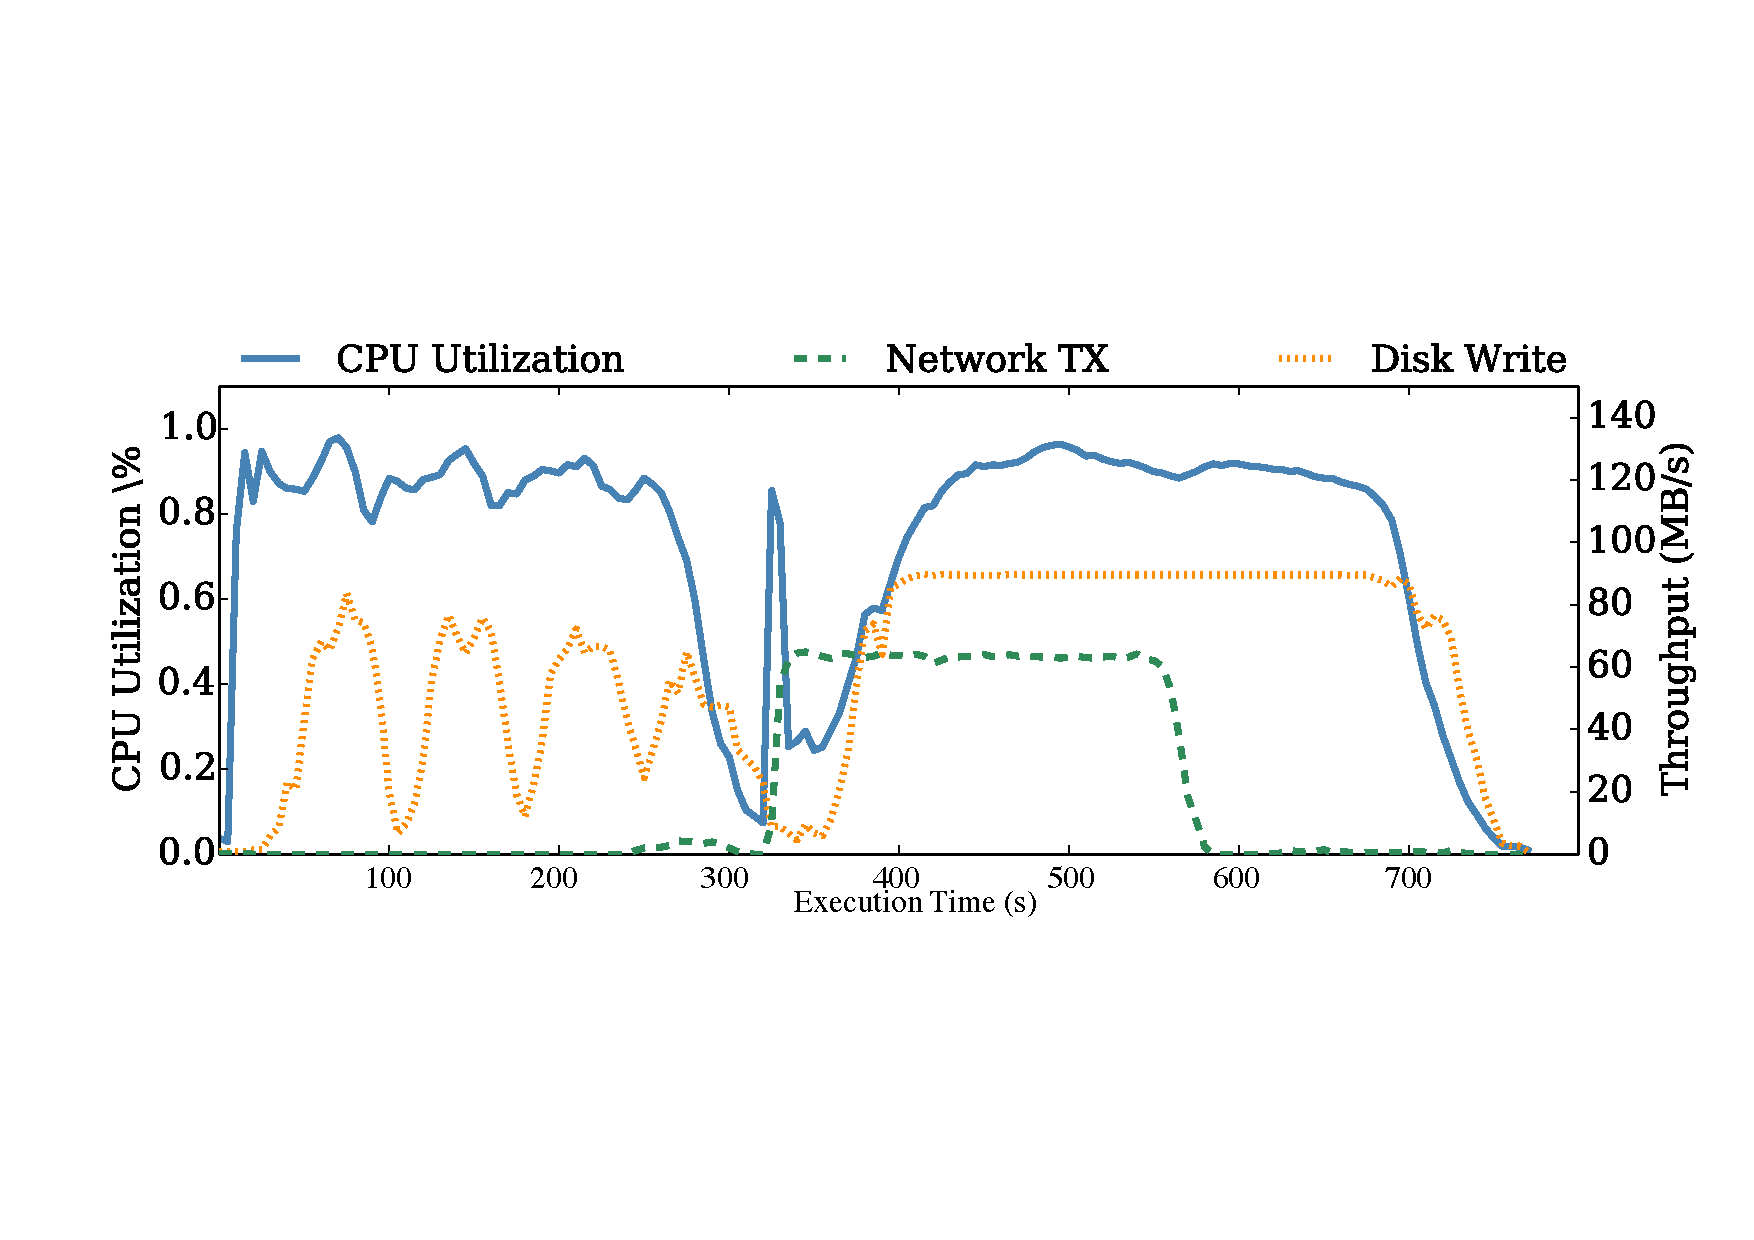
\includegraphics[width=\linewidth]{fig/hadoop_terasort_origin}
		\caption{\color{black}Hadoop MapReduce without SCache}
		\label{fig:hadoop_terasort_origin}
	\end{subfigure}
	\caption{\color{black}CPU utilization and I/O throughput of a node during a Hadoop MapReduce Terasort job}
	\label{fig:hadoop_terasort}
\end{figure}

{\color{black}
\subsection{Hadoop MapReduce with SCache}

{\color{black}
% To prove SCache compatibility as a cross-framework plug-in, we also implemented SCache on Hadoop MapReduce. 
% Although the simple DAG computing alleviates the effect of \textit{pre-scheduling}, the shuffle-heavy jobs can still be optimized by the SCache shuffle data management.
Unlike Spark, Hadoop MapReduce has only one Map and one Reduce phase.
Such a simple workflow alleviates the defect of the naive scheduling schemes and reduces the benefits of \textit{pre-scheduling}.
However, SCache can still provide considerable optimization on shuffle-heavy workloads.
We use Terasort benchmark to evaluate the performance gain of SCache and also prove the cross-framework ability of SCache.
% Although the simple workflow alleviates the benefits of \textit{pre-scheduling}, SCache can still .
% Due to the simple DAG computing in Hadoop MapReduce, we only use Terasort as a shuffle-heavy benchmark to evaluate the performance of Hadoop MapReduce with SCache.
% Figure \ref{fig:hadoop_terasort} shows the hardware resource utilization of Hadoop MapReduce running Terasort. Both figures have the same proportion of time. 
% As Figure \ref{fig:hadoop_terasort} shows, Hadoop MapReduce with SCache brings $15\%$ of total time optimization with 384GB input data size. 
}

As shown in Figure \ref{fig:hadoop_terasort_origin}, Hadoop MapReduce without SCache starts shuffle and reduce simultaneously.
% writes intermediate data locally in the map phase and the shuffle phase and the reduce phase start simultaneously.
The beginning part of reduce phase needs to wait for network transfer because a large amount of shuffle data reaches the network bottleneck.
This causes the CPU resources to be idle. 
On the other hand, in Figure \ref{fig:hadoop_terasort_scache}, Hadoop MapReduce with SCache decouples shuffle from reduce and starts pre-fetching in the map phase.
% This avoids the reduce phase waiting for the shuffle data.
SCache utilizes the idle I/O throughput in the map phase.
As shown in Figure \ref{fig:hadoop_terasort_time}, after decoupling, Hadoop MapReduce with SCache optimizes Terasort overall completion time by up to $15\%$ and an average of $13\%$ with input data sizes from 128GB to 512GB.
}

% \subsection{Overhead of Sampling}
% We evaluate the overhead of sampling with different input sizes and numbers of nodes. 
% In Figure \ref{fig:sampling}, the overhead of sampling only grows with the increase of input size on each node, but remains relatively stable when the cluster size scales up.
% Since the shuffle data is short-lived, write-once, and read-once, the central controller of SCache does not have to collect and manage complex metadata. 
% Meanwhile, most of the optimizations such as fetching and storing shuffle data are finished by workers independently. 
% So the cost of pre-scheduling algorithm and memory management are unlikely to make the master become the bottleneck of the scalability.
% Combined with the sampling overhead evaluation, we believe that SCache is scalable.

\subsection{The FRQ Model Evaluation}\label{model_evaluation}
% To evaluate the FRQ model, we run experiments on two environments: (a) 50 Amazon EC2 m4.xlarge nodes cluster; (b) 4 in-house nodes cluster with 128GB memory and 32 cores per node.
% We run the Terasort as an experimental application on a Hadoop MapReduce framework.
% We deployed Hadoop with SCache and without SCache in both environments.
To evaluate the FRQ model, we run Terasort with Hadoop MapReduce with two different environments.
%  and use the FRQ to model the jobs.
% The workload is from 16 GB to 64 GB. 
% \(D\) and \(N\) are set according to the application parameters. We set \(R, V_{Map}, V_{Shuffle},\)and \(V_{Reduce}\) according to the environment.
The parameters \(D\), \(N\), \(R\), \(V_{Map}\), \(V_{Shuffle}\), and \(V_{Reduce}\) are set according to the application and the environment.
We set \(K\) to 0.5 and 0.6 since SCache alleviates the defect on the reduce phase.
Table \ref{table1} shows the results in the in-house environment.
% The formulas of \(T_{Job}, T_{Map}, T_{Reduce}\) and \(T_{Shuffle}\) are according to Equation \ref{equation_Tjob}, Equation \ref{equation_Tmap}, Equation \ref{equation_Treduce} and Equation \ref{equation_Tshuffle}, respectively. 
While enabling SCache, Terasort satisfies the situation in Figure \ref{fig:model_basic} (\(V_{Map} \times R \ge V_{Shuffle}\)). 
% thus the formula of \(T_{P\_Shuffle}\) is Equation \ref{equation_Tpshuffle1}.
While without SCache, \(T_{P\_Shuffle}\) is equal to \(T_{Shuffle}\)(see Equation \ref{equation_Tmap}).
\(ExpT_{Job}\) represents the actual experiment job times and
\(Error\) represents the error between \(T_{Job}\) and \(ExpT_{Job}\). 
% The formula of \(Error\) is:
% \begin{equation}
% 	\label{equation_error}
% 	\begin{aligned}
% 		Error &= \frac{ExpT_{Job} - T_{Job}}{T_{Job}}
% 	\end{aligned}
% \end{equation}
Table \ref{table2} shows the results in Amazon EC2.
% \;\(V_{Map}, V_{Shuffle},\) and \(V_{Reduce}\) are modified because of the different hardware devices.
% We set K to the same value.
% The formulas in the table are all the same except \(T_{P\_Shuffle}\).
In this environment, Terasort on Hadoop MapReduce satisfies the situation in Figure \ref{fig:model_scache2} (\(V_{Map} \times R < V_{Shuffle}\)), thus the formula of \(T_{P\_Shuffle}\) is Equation \ref{equation_Tpshuffle2}. 
% In the previous case, \(T_{P\_Shuffle}\) is still equal to \(T_{Shuffle}\).

% \begin{figure}
% 	\centering
% 	\begin{subfigure}{0.49\linewidth}
% 		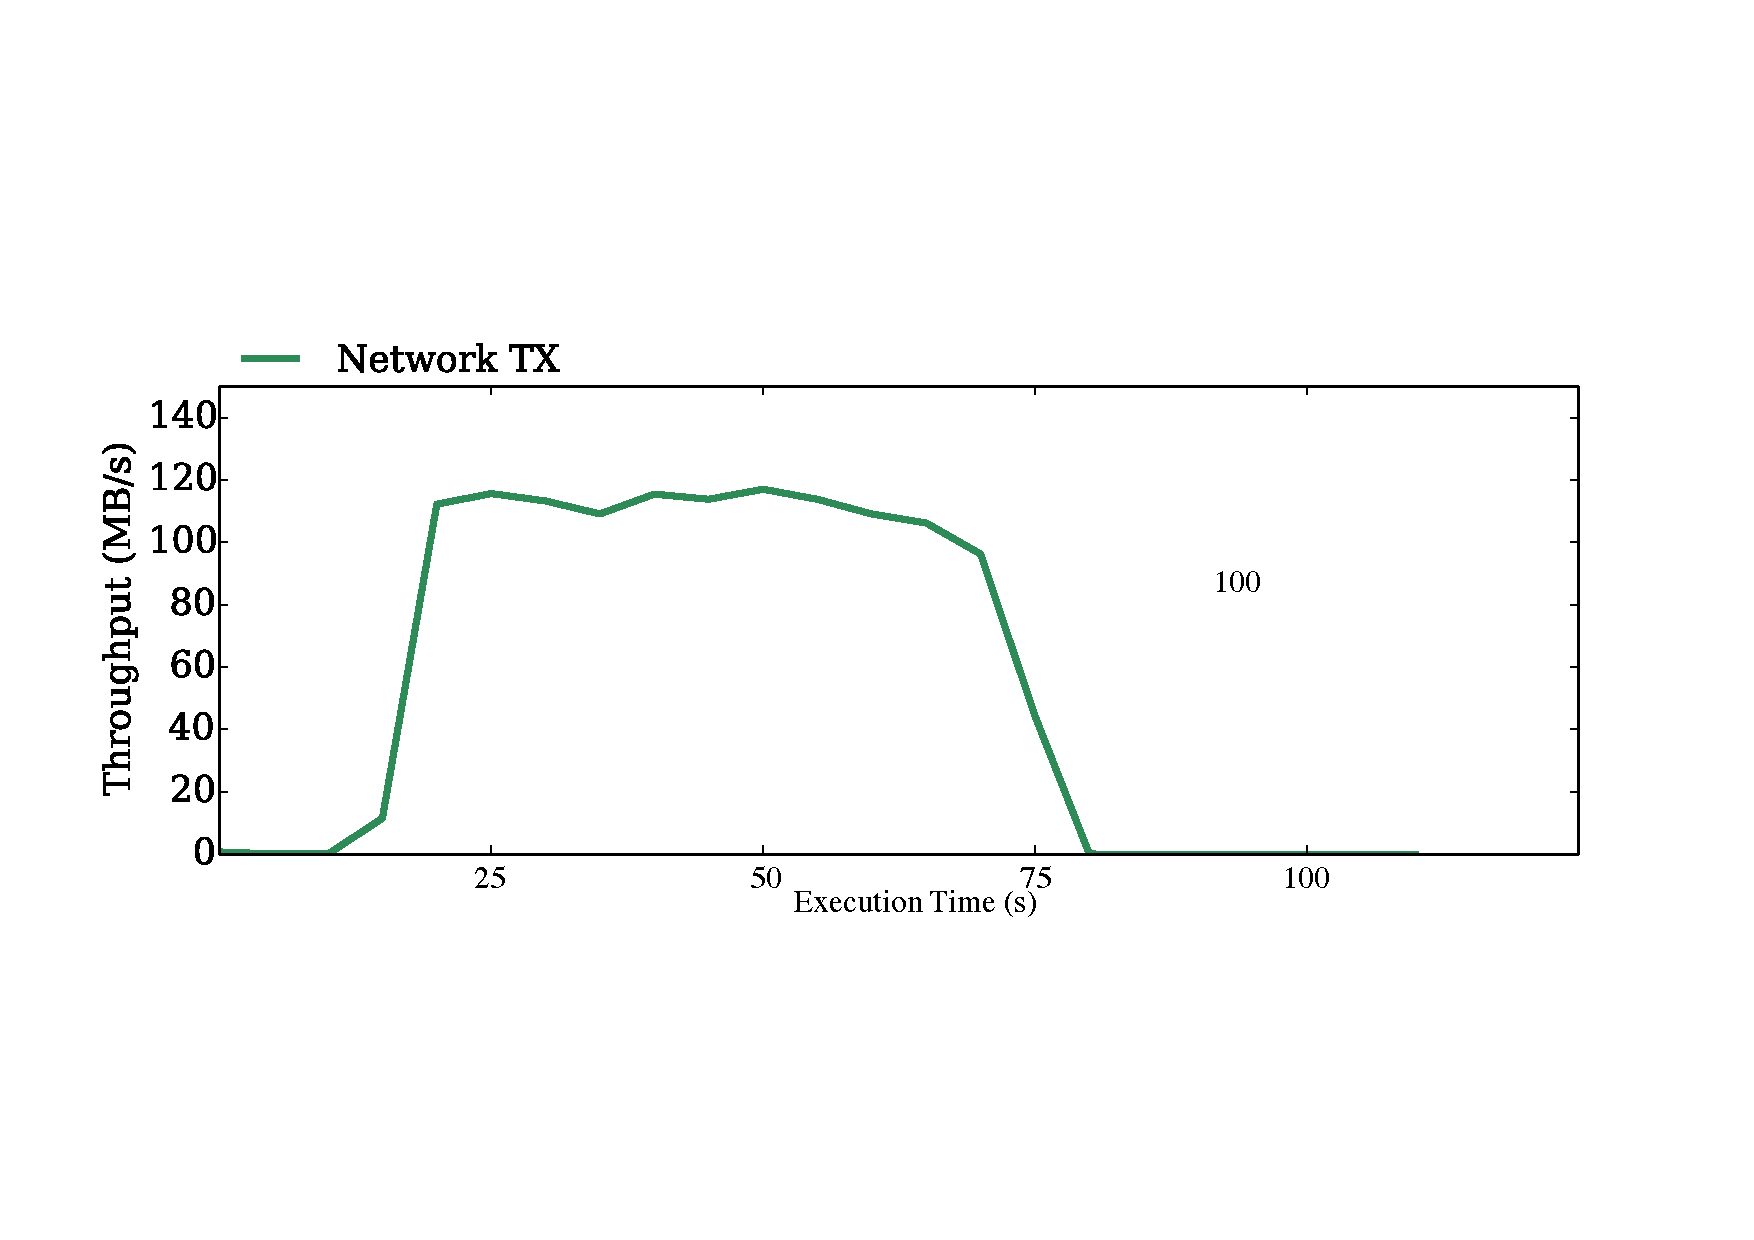
\includegraphics[width=\linewidth]{fig/hadoop_net1}
% 		\caption{\color{black}If \(V_{Map} \times R \ge V_{Shuffle}\)}
% 		\label{fig:hadoop_net1}
% 	\end{subfigure}
% 	\begin{subfigure}{0.49\linewidth}
% 		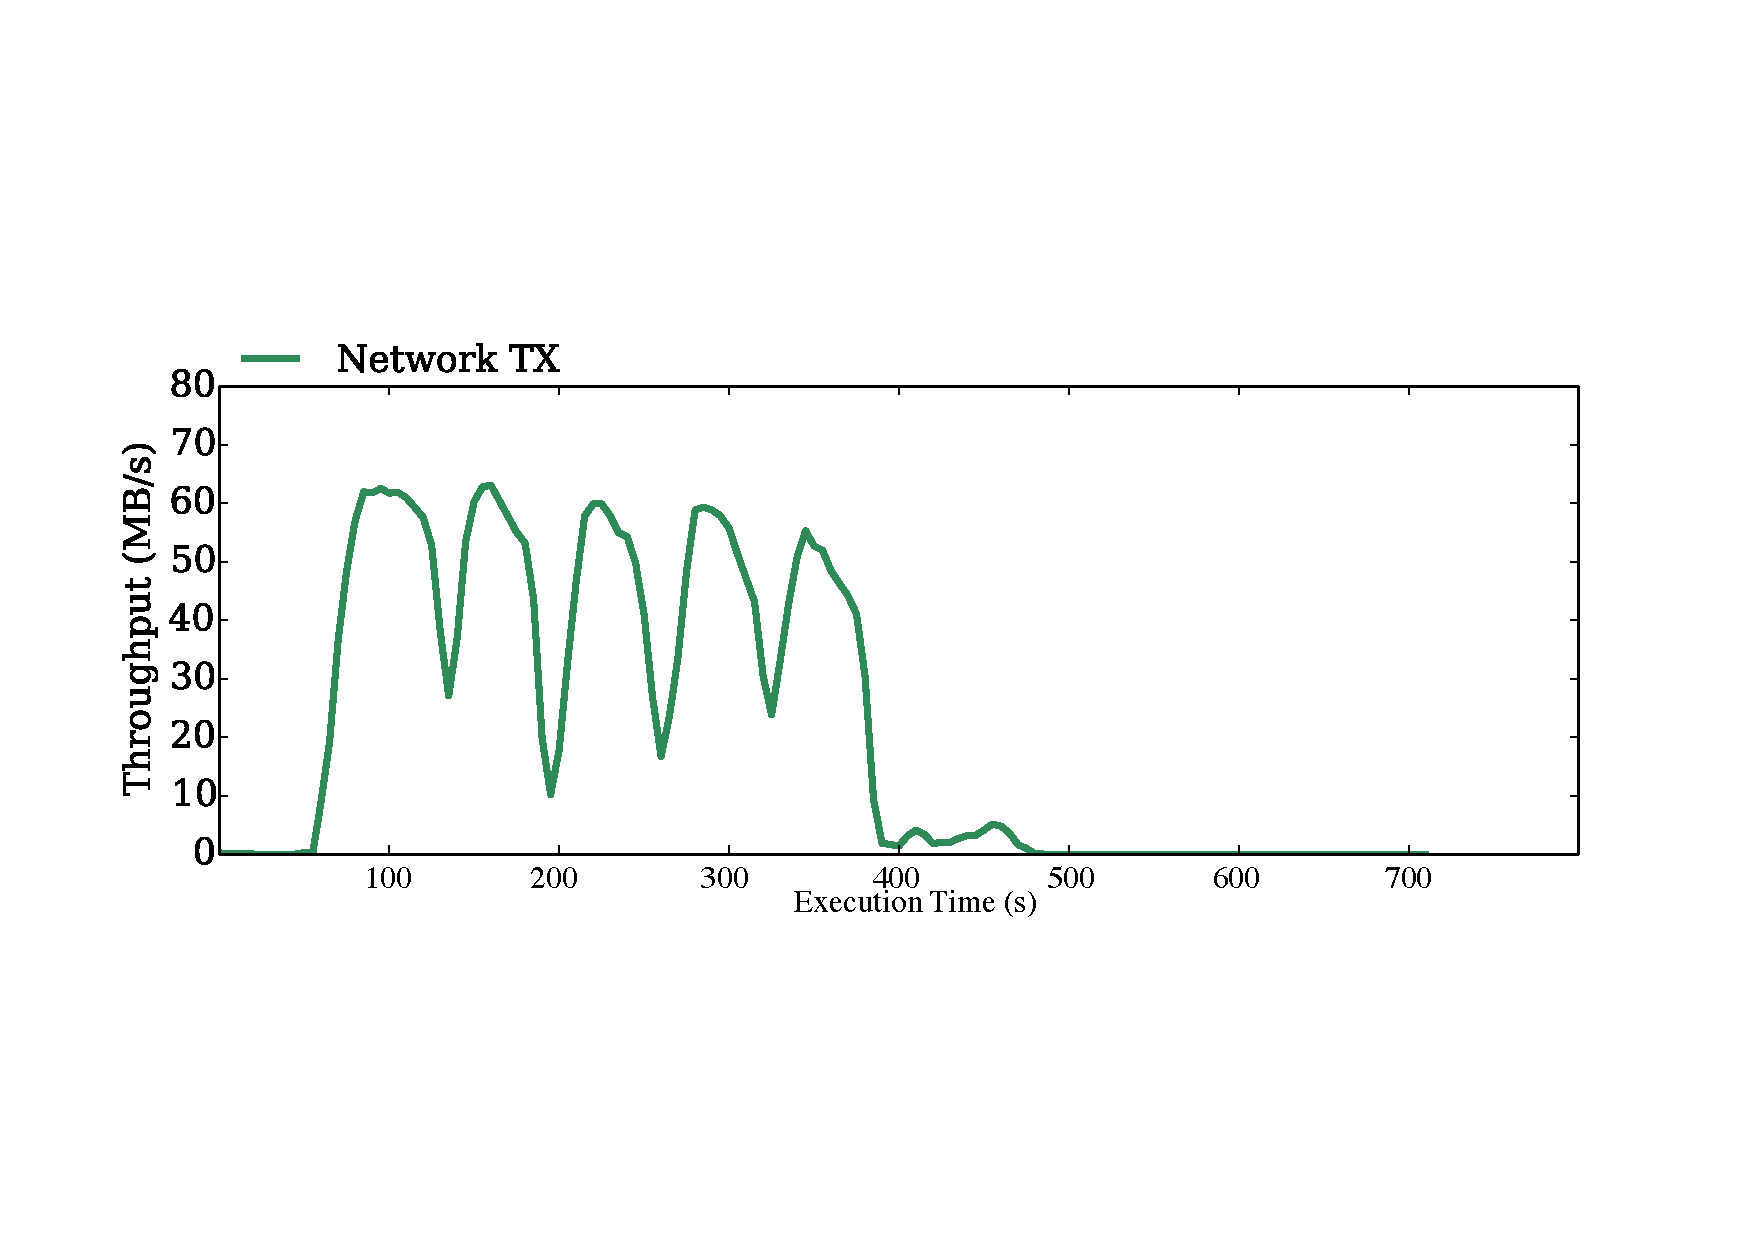
\includegraphics[width=\linewidth]{fig/hadoop_net2}
% 		\caption{\color{black}If \(V_{Map} \times R < V_{Shuffle}\)}
% 		\label{fig:hadoop_net2}
% 	\end{subfigure}
% 	\caption{\color{black}Network utilization on Hadoop MapReduce with SCache}
% 	\label{fig:hadoop_net}
% \end{figure}

% In order to evaluate the two cases as mentioned above when using SCache, we monitor the network utilization as Figure \ref{fig:hadoop_net}. Figure \ref{fig:hadoop_net1} shows that, in the in-house environment, the network utilization remains high until the shuffle phase is completed. On the other hand, Figure \ref{fig:hadoop_net2} shows that the network utilization has 5 regular peaks in Amazon EC2 environment. 
% Both these two situations are consistent with the FRQ model in Figure \ref{fig:model_scache}. 
% Therefore, we believe that the FRQ model is able to accurately describe the performance of a framework with SCache.

As shown in Table \ref{table1}\&\ref{table2}, the experimental values are all larger than the calculated values. This is because the application has some extra overhead at runtime, such as network warm-up, the overhead of allocating slots, etc. 
% In the case where the input data is small and the total time is short, the error caused by the overhead is amplified. 
This overhead will be amplified when the input data is small or the total execution time is short. 
Overall, the error between \(T_{Job}\) and \(ExpT_{Job}\) is mainly below 10\%, such errors are acceptable. 
% We believe that the FRQ model can accurately describe DAG frameworks.
}


\begin{figure}
    \centering
    \begin{minipage}{0.4\textwidth}
        \centering
        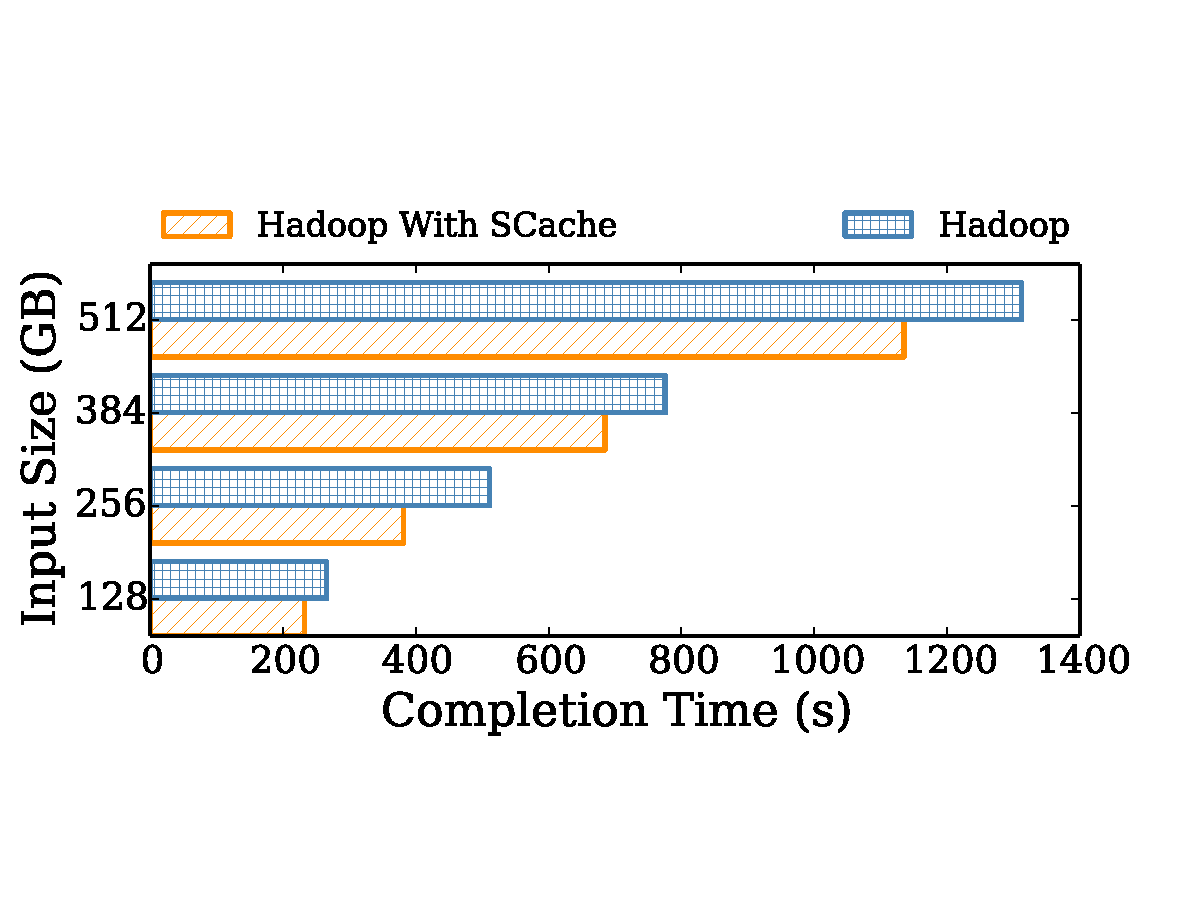
\includegraphics[width=.8\linewidth]{fig/hadoop_terasort_time} % first figure itself
        \caption{\color{black}Hadoop MapReduce Terasort Completion Time}
		\label{fig:hadoop_terasort_time}
    \end{minipage}\hfill
    % \begin{minipage}{0.4\textwidth}
    %     \centering
    %     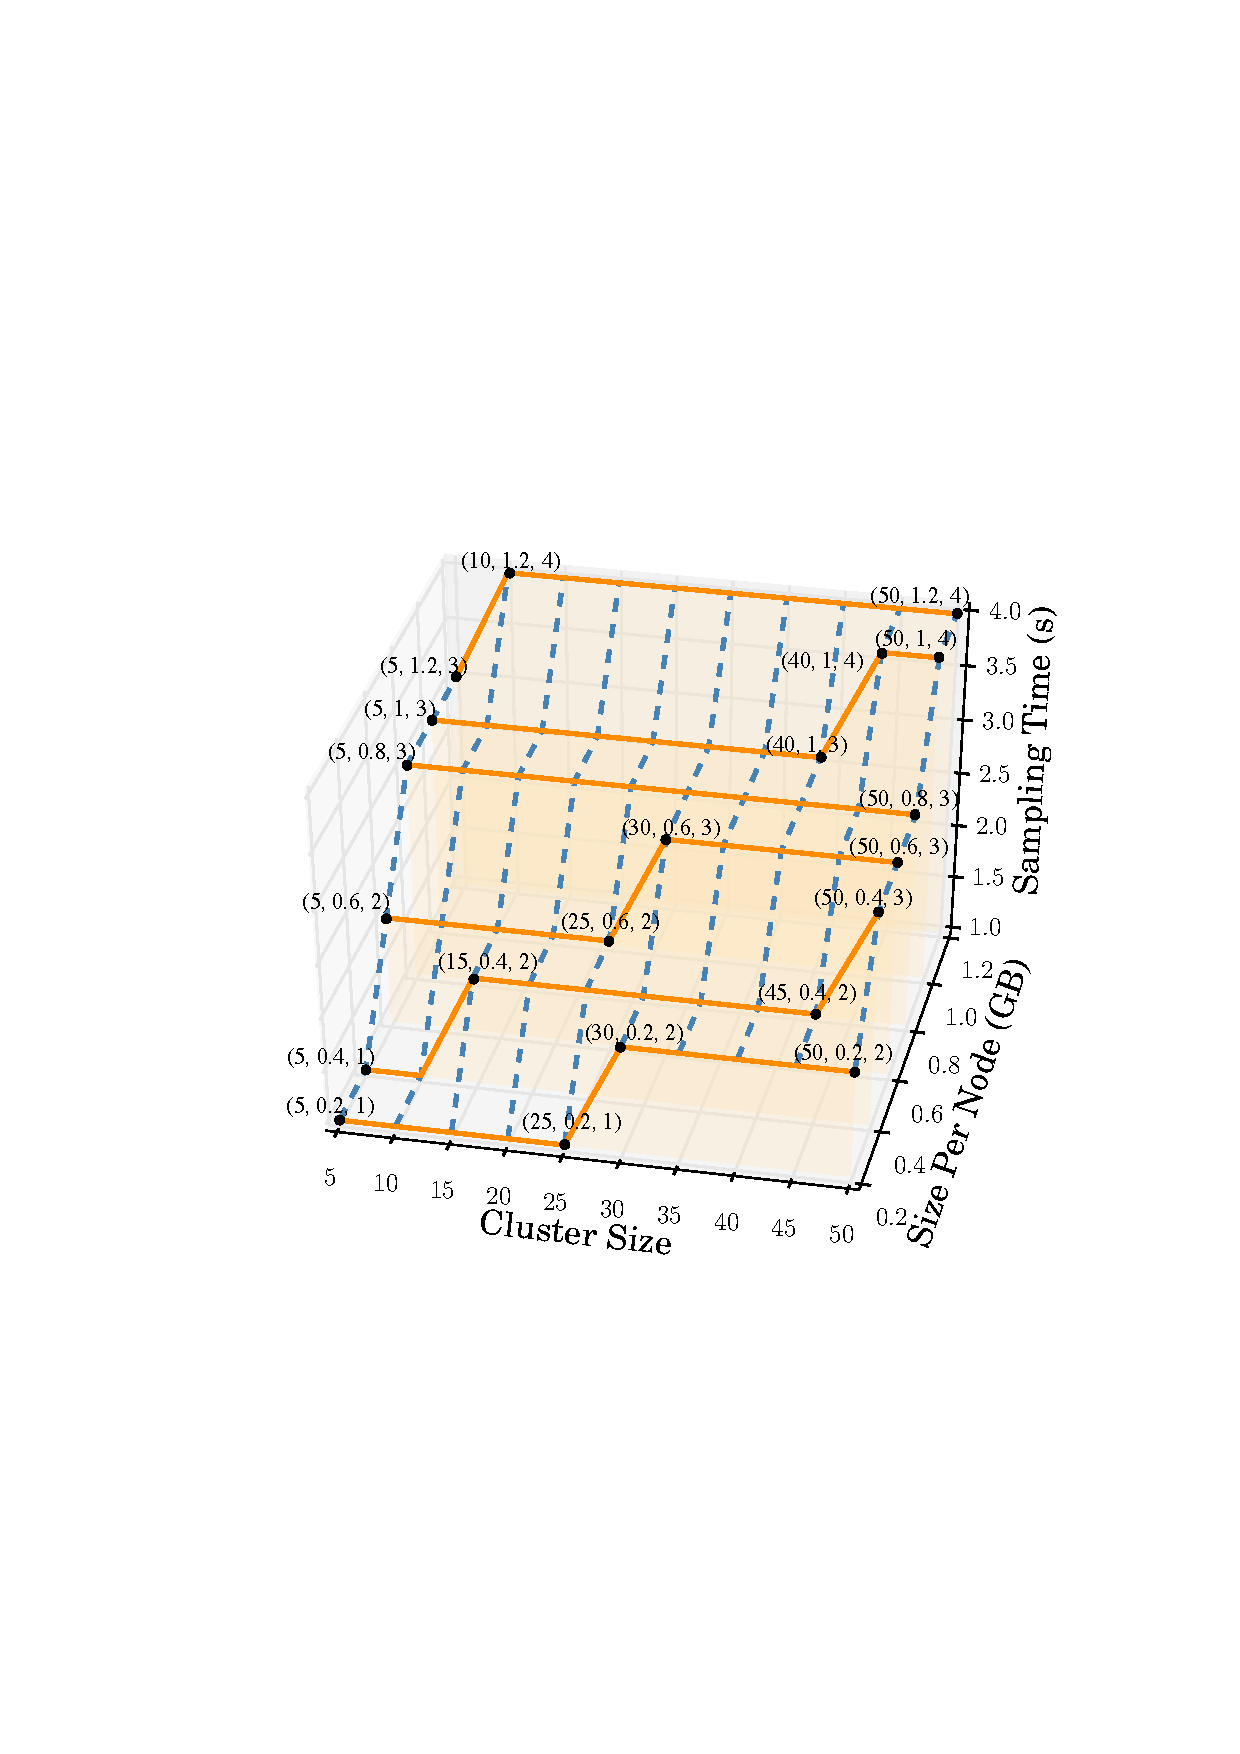
\includegraphics[width=.8\linewidth]{fig/sampling} % second figure itself
    %     \caption{Sampling Overhead}
	% 	\label{fig:sampling}
    % \end{minipage}
\end{figure}

\begin{table*}
\centering
\scalebox{0.85}{
	\begin{tabular}{|c||c|c|c|c|c|c|c||c|c|c|c|c|c|c|}
	\hline
	&
	\(D\) &	
	\(R\) &	
	\(N\) &	
	\(V_{Map}\) &	
	\(V_{Reduce}\) &	
	\(V_{Shuffle}\) &	
	\(K\) &	
	\(T_{Map}\) &	
	\(T_{Shuffle}\) &	
	\(T_{P\_Shuffle}\) &
	\(T_{Reduce}\) & 
	\(T_{Job}\) & 
	\(Exp T_{Job}\) &
	\(Error\)\\

	\hline
	% & 16	& 1	& 2 &	0.65 &	1 &	0.47 &	0.5 &	24.62 &		34.04	 &	21.73 &	26.87 &	51.48	& 55  &		6.39\% \\
	SCache
	& 32 GB & 1	& 4 &	0.65 GB/s &	1 GB/s  &	0.47 GB/s &	0.5 &	49.23 &		68.09  s &	31.16 s &	47.58 s &	96.81	s & 104 s & 	6.91\% \\
	& 48 GB	& 1	& 6 &	0.65 GB/s &	1 GB/s  &	0.47 GB/s &	0.5 &	73.85 &		102.13 s &	40.59 s &	68.29 s &	142.14	s & 151 s & 	5.87\% \\
	& 64 GB	& 1	& 8 &	0.65 GB/s &	1 GB/s  &	0.47 GB/s &	0.5 &	98.46 &		136.17 s &	50.02 s &	89.01 s &	187.47	s & 193 s & 	2.87\% \\
	\hline
	% & 16	& 1 & 2 &	0.65 GB/s &	1 &	0.47 &	0.6 &	24.62 &		34.04	&	34.04	&	36.43	&	61.04	&	73	&	16.38\%	\\
	Legacy
	& 32 GB	& 1 & 4 &	0.65 GB/s &	1 GB/s &	0.47 GB/s &	0.6 &	49.23 s &		68.09 s &	68.09 s		&	72.85	s &	122.08 s	&	135 s	&	9.57\%	\\
	& 48 GB	& 1 & 6 &	0.65 GB/s &	1 GB/s &	0.47 GB/s &	0.6 &	73.85 s &		102.13 s &	102.13 s	&	109.28	s &	183.12 s	&	188 s	&	2.59\%	\\
	& 64 GB	& 1 & 8 &	0.65 GB/s &	1 GB/s &	0.47 GB/s &	0.6 &	98.46 s &		136.17 s &	136.17 s	&	145.70	s &	244.16 s	&	249 s	&	1.94\%	\\
	\hline
	\end{tabular}
}
% \(D\): GB, \(V_{i}\): GB/s, \(T_{i}\): s
\caption{\color{black}Hadoop MapReduce on 4 nodes cluster in the FRQ model}
\label{table1}
\end{table*}

% \subsection{Performance Analysis}\label{model_performance_analysis}

% \begin{table*}[!t]

\begin{table*}
\centering
\scalebox{0.85}{
	\begin{tabular}{|c||c|c|c|c|c|c|c||c|c|c|c|c|c|c|}
	\hline
	&
	\(D\) &	
	\(R\) &	
	\(N\) &	
	\(V_{Map}\) &	
	\(V_{Reduce}\) &	
	\(V_{Shuffle}\) &	
	\(K\) &	
	\(T_{Map}\) &	
	\(T_{Shuffle}\) &	
	\(T_{P\_Shuffle}\) &
	\(T_{Reduce}\) & 
	\(T_{Job}\) & 
	\(Exp T_{Job}\) &
	\(Error\)\\

	\hline
	SCache
	& 128 GB	& 1 & 5 &	1.15 GB/s &	1.46 GB/s	&	1.4 GB/s &	0.5 &	111.30 &	91.43	&	18.29	&	96.81	&	208.12	&	232	&	10.29\%	\\
	& 256 GB	& 1 & 5 &	1.15 GB/s &	1.46 GB/s	&	1.4 GB/s &	0.5 &	222.61 &	182.86	&	36.57	&	193.63	&	416.24	&	432	&	3.65\%	\\
	& 384 GB	& 1 & 5 &	1.15 GB/s &	1.46 GB/s	&	1.4 GB/s &	0.5 &	333.91 &	274.29	&	54.86	&	290.44	&	624.36	&	685 &	8.85\%	\\
	% & 512	& 1 & 5 &	1.15 GB/s &	1.46 GB/s	&	1.4 GB/s &	0.5 &	445.22 &	365.71	&	91.43	&			&	841.62	&	1135 &	25.85\%	\\
	\hline
	Legacy
	& 128 GB	& 1 & 5 &	1.15 GB/s &	1.46 GB/s	&	1.4 GB/s &	0.6 &	111.30 s &	91.43	s &	91.43	s &	142.53	s &	253.83	s &	266 s &	4.57\%	\\
	& 256 GB	& 1 & 5 &	1.15 GB/s &	1.46 GB/s	&	1.4 GB/s &	0.6 &	222.61 s &	182.86	s &	182.86	s &	285.06	s &	507.67	s &	524 s &	3.12\%	\\
	& 384 GB	& 1 & 5 &	1.15 GB/s &	1.46 GB/s	&	1.4 GB/s &	0.6 &	333.91 s &	274.29	s &	274.29	s &	427.59	s &	761.50	s &	776 s &	1.87\%	\\
	% & 512	& 1 & 5 &	1.15 &	1.46	&	1.4 &	0.6 &	445.22 &	365.71	&	365.71	&	588.40	&	1033.62	&	1312 &	21.22\%	\\

	\hline
	\end{tabular}
}
% \(D\): GB, \(V_{i}\): GB/s, \(T_{i}\): s
\caption{\color{black}Hadoop MapReduce on 50 AWS m4.xlarge nodes cluster in the FRQ model}
\label{table2}
\end{table*}